% !TEX root = main.tex

\subsection{控制单元}
\label{sub:control_unit}
\qquad 多周期CPU最重要的一点在于状态转移的分析,如图\ref{fig:state}所示。
\begin{figure}[H]
\centering
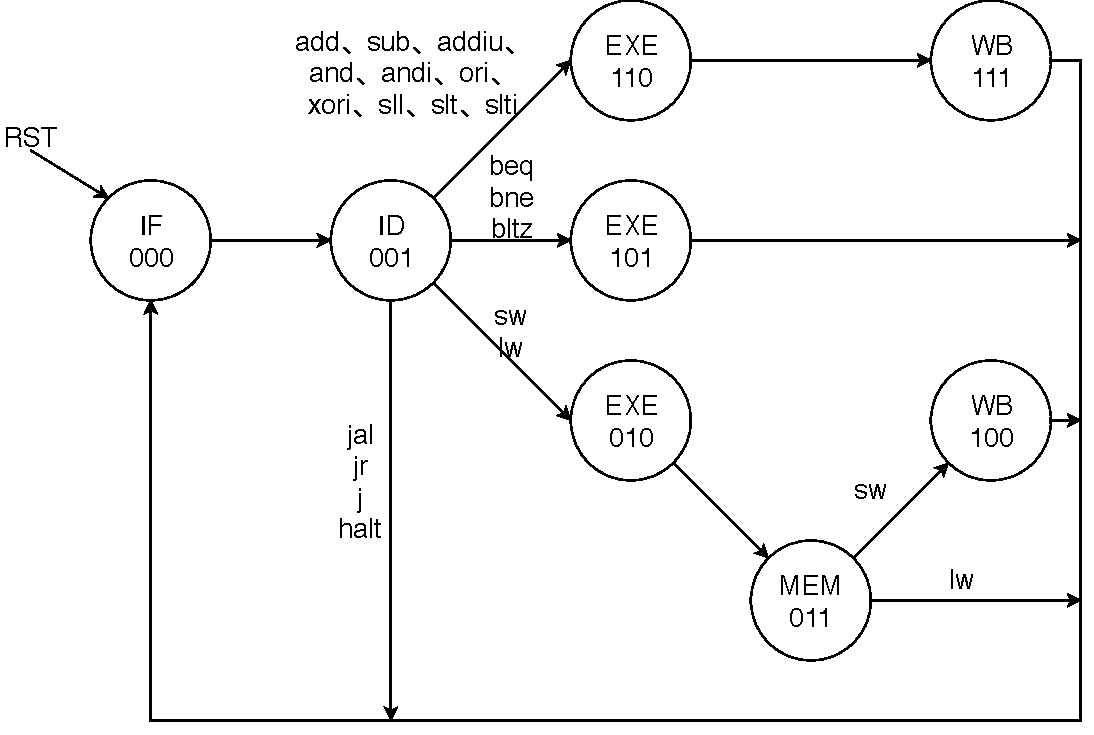
\includegraphics[width=0.65\linewidth]{fig/State.pdf}
\caption{多周期CPU状态转移图}
\label{fig:state}
\end{figure}
\par 由前面的分析,可以得到控制单元的编码表,见表\ref{tab:control_codes}。
\textcolor{red}{注意表\ref{tab:control_codes}仅仅指明了一条指令的执行过程中全部控制信号的取值,具体到各个阶段,则需结合当前状态判断控制信号是否有效。如只在IF阶段允许PC的修改,即PCWrite为1;而只在WB阶段可以进行寄存器的写操作,即RegWr为1。具体实现参见第\ref{sec:appendix}章控制单元一节。}
% Table generated by Excel2LaTeX from sheet 'TrueTable'
\begin{sidewaystable}[htbp]
  \centering\xiaowu
  \caption{指令控制器编码}
    \begin{tabular}{|c|l|l|r|r|r|cc|r|r|r|r|r|r|}
    \hline
          & \multicolumn{1}{c|}{指令} & \multicolumn{1}{c|}{op} & \multicolumn{1}{c|}{RegDst} & \multicolumn{1}{c|}{ExtSel} & \multicolumn{1}{c|}{RegWrite} & \multicolumn{2}{c|}{ALUSrcA/B} & \multicolumn{1}{c|}{ALUOp} & \multicolumn{1}{c|}{DBSrc} & \multicolumn{1}{c|}{WrRegSrc} & \multicolumn{1}{c|}{MemWrite} & \multicolumn{1}{c|}{PCSrc} & \multicolumn{1}{c|}{PCWrite} \bigstrut\\
    \hline
    \multirow{3}[6]{*}{算术运算} & add rd, rs, rt & 000000 & 1     & x     & 1     & \multicolumn{2}{c|}{00} & 000   & 0     & 0     & 0     & 00    & 1 \bigstrut\\
\cline{2-14}          & sub rd, rs, rt & 000001 & 1     & x     & 1     & \multicolumn{2}{c|}{00} & 001   & 0     & 0     & 0     & 00    & 1 \bigstrut\\
\cline{2-14}          & addiu rt, rs, imm & 000010 & 0     & \textbf{1} & 1     & \multicolumn{2}{c|}{01} & 000   & 0     & 0     & 0     & 00    & 1 \bigstrut\\
    \hline
    \multirow{4}[8]{*}{逻辑运算} & and rd, rs, rt & 010000 & 1     & x     & 1     & \multicolumn{2}{c|}{00} & 100   & 0     & 0     & 0     & 00    & 1 \bigstrut\\
\cline{2-14}          & andi rt, rs, imm & 010001 & 0     & 0     & 1     & \multicolumn{2}{c|}{01} & 100   & 0     & 0     & 0     & 00    & 1 \bigstrut\\
\cline{2-14}          & ori rt, rs, imm & 010010 & 0     & 0     & 1     & \multicolumn{2}{c|}{01} & 011   & 0     & 0     & 0     & 00    & 1 \bigstrut\\
\cline{2-14}          & \textbf{xori rt, rs, imm} & 010011 & 0     & 0     & 1     & \multicolumn{2}{c|}{01} & 111   & 0     & 0     & 0     & 00    & 1 \bigstrut\\
    \hline
    移位    & sll rd, rt, sa & 011000 & 1     & x     & 1     & \multicolumn{2}{c|}{10} & 010   & 0     & 0     & 0     & 00    & 1 \bigstrut\\
    \hline
    \multirow{2}[4]{*}{比较} & slti rt, rs, imm & 100110 & 0     & 1     & 1     & \multicolumn{2}{c|}{01} & 110   & 0     & 0     & 0     & 00    & 1 \bigstrut\\
\cline{2-14}          & \textbf{slt rd, rs, rt} & 100111 & 1     & x     & 1     & \multicolumn{2}{c|}{00} & 110   & 0     & 0     & 0     & 00    & 1 \bigstrut\\
    \hline
    \multirow{2}[4]{*}{访存} & sw rt, imm(rs) & 110000 & x     & 1     & 0     & \multicolumn{2}{c|}{01} & 000   & x     & 0     & 1     & 00    & 1 \bigstrut\\
\cline{2-14}          & lw rt, imm(rs) & 110001 & 0     & 1     & 1     & \multicolumn{2}{c|}{01} & 000   & 1     & 0     & 0     & 00    & 1 \bigstrut\\
    \hline
    \multirow{3}[6]{*}{分支} & beq rs, rt, imm & 110100 & x     & 1     & 0     & \multicolumn{2}{c|}{00} & 001   & x     & 0     & 0     & 10    & 1 \bigstrut\\
\cline{2-14}          & bne rs, rt, imm & 110101 & x     & 1     & 0     & \multicolumn{2}{c|}{00} & 001   & x     & 0     & 0     & 10    & 1 \bigstrut\\
\cline{2-14}          & bltz rs, imm & 110110 & x     & 1     & 0     & \multicolumn{2}{c|}{00} & 110   & x     & 0     & 0     & 10    & 1 \bigstrut\\
    \hline
    \multirow{2}[4]{*}{跳转} & j addr & 111000 & x     & x     & 0     & \multicolumn{2}{c|}{xx} & x     & x     & 0     & 0     & 01    & 1 \bigstrut\\
\cline{2-14}          & \textbf{jr rs} & 111001 & x     & x     & 0     & \multicolumn{2}{c|}{0x} & x     & x     & 0     & 0     & 11    & 1 \bigstrut\\
    \hline
    调用子程序 & \textbf{jal addr} & 111010 & \textbf{2} & x     & \textbf{1} & \multicolumn{2}{c|}{xx} & x     & x     & \textbf{1} & 0     & 01    & 1 \bigstrut\\
    \hline
    停机    & halt  & 111111 & x     & x     & 0     & \multicolumn{2}{c|}{xx} & x     & x     & x     & 0     & xx    & 0 \bigstrut\\
    \hline
    \end{tabular}%
  \label{tab:control_codes}%
\end{sidewaystable}%